En este caítulo se presentan los avances que se tienen del sistema en análisis y diseño por cada sprint ...

\section{Sprits del proyecto}
En casi todos sprints se cubren requerimientos funcionales del sistema, estos requerimientos utilizan una 
clave para ser identificados:

\begin{itemize}
	\item Para los requerimientos \textbf{fucionales} se utliza el formato \textbf{RF-X}, donde:
    \begin{itemize}
        \item \textbf{RF} Es la clave para todos los requerimientos funcionales.
        \item \textbf{X} Es un número consecutivo: 01, 02, 03, ...
    \end{itemize}

    \item Para los requerimientos \textbf{no fucionales} se utliza el formato \textbf{RNF-X}, donde:
    \begin{itemize}
        \item \textbf{RNF} Es la clave para todos los requerimientos funcionales.
        \item \textbf{X} Es un número consecutivo: 01, 02, 03, ...
    \end{itemize}
\end{itemize}

\subsection{Sprint 1: Pruebas de concepto}
Esta iteración tuvo como propósito capacitarnos en las tecnologías que se van ha estar utilizando 
a lo largo del desarrollo del sistema.La actividades que se realizaron las siguientes:

\begin{enumerate}
    \item Crear el product backlog así como elementos de apoyo para dar prioridad y seguimiento.
    \item Especificar el lugar físico en el que el código del proyecto se va almacenar y que permita que
    todos los miembros del equipo puedan darle mantenimiento.
    \item Configurar las diferentes plataformas y tecnologías necesarias para el proyecto.
\end{enumerate}

\subsection{Sprint 2: Análisis y planificación general del sistema}
Esta iteración tuvo como establecer los fundamentos teóricos y prácticos para su desarrollo.Las actividades que se realizaron 
de manera general fueron las siguientes:
\begin{enumerate}
    \item Se hizo el levantamiento de requerimientos a travez de juntas con el personal de la bolsa de trabajo de ESCOM.
    \item Se adquirieron las licencias de Balsamiq Cloud y Visual Paradigm  para todo el análisis de
    requerimientos y de diseño.
    \item Se creo un repositorio usando el Sistema de Control de Versiones Git para almacenar el código y la documentación del proyecto
    utilizando la prataforma de GitHub.
    \item Se configuró el proyecto en front end utilizando React Js con la versión 17.0.2.
\end{enumerate} 


\subsection{Sprint 3: Gestión de Usuarios}
Esta iteración tuvo como propósito implementar un mecanismo que permita a los usuarios del sistema autenticarse y/o crear cuentas
para acceder al mismo, las actividades realizadas fueron:
\begin{enumerate}
    \item Se diseñó e implementó las interfaces de usuario para la gestión de cuentas y accesos.
    \item Se especificaron los requerimientos mediante casos de uso con sus respectivas interfaces de usuario.
    \item Se elaboró el a de casos de uso para este sprint.
    \item Se elaboró la maquina de estados de un reclutador.
\end{enumerate} 

Los requerimientos funcionales de este sprint se muestran en la siguiente tabla.
\begin{requerimientos}{funcionales}
    \RFitem{RF-01}{Iniciar sesión }{El sistema debe proporcionar un mecanismo que permita al actor acceder al sistema mediante un correo y una contraseña.}
    \RFitem{RF-02}{Crear cuenta}{El sistema debe proporcionar un mecanismo que permita al actor registrarse como nuevo usuario en el sistema.}
    \RFitem{RF-04}{Consultar perfil}{El sistema debe permitir al actor acceder a su perfil para consultar la información registrada.}
    \RFitem{RF-05}{Editar perfil}{El sistema debe permitir al actor modificar la información registrada en su perfil, como nombre, apellidos, información de contacto y si el usuario es un candidato, debe de permitir modificar su información académica y datos de habilidades y conocimientos del mismo.}
    \RFitem{RF-24}{Enviar solicitud para acceder al sistema}{El sistema debe proporcionar un mecanismo para que al representante de una empresa pueda enviar una solicitud o pre-registro de poder acceder y publicar vacantes.}
\end{requerimientos}

Los casos de uso que se implementaron en este sprint fueron:
\begin{enumerate}
    \item \refElem{GRL-CU01}
    \item \refElem{GRL-CU02}
    \item \refElem{GRL-CU03}
    %\item \refElem{USR-CU02-2}
\end{enumerate} 


\subsection{Sprint 4: Gestión de Vacantes}

Esta iteración tuvo como propósito implementar un mecanismo para la gestión de vacantes dentro del sistema, las actividades 
realizadas fueron:
\begin{enumerate}
    \item Se diseñó e implementó las interfaces de usuario para la gestión de vacantes ú el tipo de cuenta.
    \item Se especificaron los requerimientos mediante casos de uso con sus respectivas interfaces de usuario.
    \item Se elaboró el a de casos de uso para este sprint.
    \item Se elaboró la maquina de estados de una vacante.
\end{enumerate} 

Los requerimientos funcionales de este sprint se muestran en la siguiente tabla.
\begin{requerimientos}{funcionales}
    \RFitem{RF-09}{Consultar vacantes}{El sistema debe permitir a cualquier persona consultar las vacantes que se tengan registradas siempre y cuando aun estén abiertas.}
    \RFitem{RF-10}{Publicar vacantes }{El sistema debe permitir  a los usuarios registrados publicar vacantes.}
    \RFitem{RF-11}{Editar vacantes}{El sistema debe permitir a los usuarios editar las vacantes que ellos hayan publicado.}
    \RFitem{RF-12}{Reportar vacantes}{El sistema debe permitir a los usuarios reportar vacantes publicadas si es que el usuario lo crea necesario.}
    \RFitem{RF-13}{Eliminar vacantes}{El sistema debe permitir a los usuarios eliminar las vacantes que ellos hayan publicado.}
\end{requerimientos}

Los casos de uso que se implementaron en este sprint fueron:
\begin{enumerate}
    \item VCT-CU01 Buscar vacantes
    \item VCT-CU03-1 Cerrar vacante
    \item VCT-CU06 Listar vacantes
    \item VCT-CU06-1 Consultar vacante
    \item VCT-CU03-2 Editar vacante
    \item VCT-CU03-3 Elimnar vacante
    \item VCT-CU03 Publicar vacante
\end{enumerate} 



\subsection{Sprint 5: Gestión de Postulaciones}

Esta iteración tuvo como propósito implementar un mecanismo para gestionar las postulaciones de los usuarios registrdos dentro del 
sistema, las actividades realizadas fueron:
\begin{enumerate}
    \item Se diseñó e implementó las interfaces de usuario para la gestión de posutlaciones según el tipo de cuenta.
    \item Se especificaron los requerimientos mediante casos de uso con sus respectivas interfaces de usuario.
    \item Se elaboró el diagrama de casos de uso para este sprint.
    \item Se elaboró la maquina de estados de una postulaciones.
\end{enumerate} 

Los requerimientos funcionales de este sprint se muestran en la siguiente tabla.
\begin{requerimientos}{funcionales}
    \RFitem{RF-14}{Postularse a vacantes}{El sistema debe permitir a los usuarios registrados enviar postularse a  las vacantes que esté abiertas.}
    \RFitem{RF-15}{Consultar el estado de postulaciones}{El sistema debe permitir al actor consultar el estado de su o sus postulaciones que haya hecho.}
    \RFitem{RF-16}{Dar seguimiento a postulaciones}{El sistema debe permitir al actor indicar  el estado de las postulaciones que tiene según sus vacantes publicadas.}
    \RFitem{RF-17}{Consultar postulaciones}{El sistema debe permitir a los actores registrados consultar las postulaciones que se hayan hecho de acuerdo a cada vacante.}
        
\end{requerimientos}


Los casos de uso que se implementaron en este sprint fueron:
\begin{enumerate}
    \item PST-CU1 Consultar postulaciones
    \item PST-CU2 Postularse a una vacante
    \item PST-CU1-2 Rechazar postulación
\end{enumerate} 


\section{Casos de uso}


%\begin{UseCase}[]{USR-CU03.3}{ELiminar Idioma}{
	%Permite al alumno consultar la información de sus idiomas registrados en el perfil.
}
	%----------------------------------------------------------------
	% Datos generales del CU:
	\UCsection{Atributos}
	\UCitem{Actor(es)}{
		\Titem Candidato. 
	}
	\UCitem[admin]{Prioridad}{ 
		\Titem Media.
	}
	\UCitem[admin]{Complejidad}{
		\Titem Baja
	}
	\UCitem{Precondiciones}{
		\Titem El alumno debe de tener una cuenta en el sistema.
		\Titem Se debe de tener previmante registrado al menos un idioma.
	}
	\UCitem{Destino}{
		\Titem \refElem{USR-IU03.1}
	}
	\UCitem{Reglas de Negocio}{
		\Titem Ninguna.
		
	}
	\UCitem{Viene de}{
		\Titem Caso de uso \refIdElem{USR-CU03}.
	}	
\end{UseCase}

%Trayectoria Principal
\begin{UCtrayectoria}
	\UCpaso [\UCactor] Presiona el botón \IUEliminar{} desde la interfaz \refElem{USR-IU03}.
    \UCpaso [\UCsist] Muestra la interfaz \refElem{USR-IU03.3}.
	\UCpaso [\UCactor] Presiona el botón \IUbutton{Aceptar}.\refTray{A}
	\UCpaso [\UCsist] Agrega al catalogo de idiomas el idioma que se quiere eliminar.
	\UCpaso [\UCsist] Eliminar el registro del idioma en el sistem.
	\UCpaso [\UCsist] Muestra la información actualizada en la interfaz \refElem{USR-IU03}.
\end{UCtrayectoria}

\begin{UCtrayectoriaA}[Fin del caso de uso]{A}{El actor desea cancelar el registro}
	\UCpaso [\UCsist] Presiona el botón \IUbutton{Cancelar}.
	\extendUC{USR-CU03}.
\end{UCtrayectoriaA} 


%\begin{UseCase}[]{USR-CU03.3}{ELiminar Idioma}{
	%Permite al alumno consultar la información de sus idiomas registrados en el perfil.
}
	%----------------------------------------------------------------
	% Datos generales del CU:
	\UCsection{Atributos}
	\UCitem{Actor(es)}{
		\Titem Candidato. 
	}
	\UCitem[admin]{Prioridad}{ 
		\Titem Media.
	}
	\UCitem[admin]{Complejidad}{
		\Titem Baja
	}
	\UCitem{Precondiciones}{
		\Titem El alumno debe de tener una cuenta en el sistema.
		\Titem Se debe de tener previmante registrado al menos un idioma.
	}
	\UCitem{Destino}{
		\Titem \refElem{USR-IU03.1}
	}
	\UCitem{Reglas de Negocio}{
		\Titem Ninguna.
		
	}
	\UCitem{Viene de}{
		\Titem Caso de uso \refIdElem{USR-CU03}.
	}	
\end{UseCase}

%Trayectoria Principal
\begin{UCtrayectoria}
	\UCpaso [\UCactor] Presiona el botón \IUEliminar{} desde la interfaz \refElem{USR-IU03}.
    \UCpaso [\UCsist] Muestra la interfaz \refElem{USR-IU03.3}.
	\UCpaso [\UCactor] Presiona el botón \IUbutton{Aceptar}.\refTray{A}
	\UCpaso [\UCsist] Agrega al catalogo de idiomas el idioma que se quiere eliminar.
	\UCpaso [\UCsist] Eliminar el registro del idioma en el sistem.
	\UCpaso [\UCsist] Muestra la información actualizada en la interfaz \refElem{USR-IU03}.
\end{UCtrayectoria}

\begin{UCtrayectoriaA}[Fin del caso de uso]{A}{El actor desea cancelar el registro}
	\UCpaso [\UCsist] Presiona el botón \IUbutton{Cancelar}.
	\extendUC{USR-CU03}.
\end{UCtrayectoriaA} 


%\clearpage
\subsection{USR-IU02.2 Editar Medios de contacto y redes sociales}

\subsubsection{Objetivo}
En la figura \refElem{USR-IU02.2} se muestra la interfaz correspondiente con la funcionalidad descrita en las
trayectorias del caso de uso \refElem{USR-CU02.2} , la cual permite al actor editar sus medios de contacto como son: correos, teléfonos y redes sociales.

\subsubsection{Comandos}
Los siguientes comandos aparecen en la interfaz descrita anteriormente.
\Titem \IUbutton{Aceptar} : Cuando presiona el botón, actualiza la información .
\Titem \IUbutton{Cancelar} : Cuando presiona el botón, muestra la sección anterior.%\refElem{GRL-IU02-2}.

\IUfig{.9}{CasosdeUso/USR-CU02-2/imagenes/USR-IU02.2.png}{USR-IU02.2}{Editar Medios de contacto y redes sociales}  


\clearpage


Los casos de uso son una herramienta usada para representar las transacciones entre un actor y el sistema, las cuales siempre tendrán un valor agregado o un propósito para que el actor las realice.
En estos se representan a traves de aas los cuales se conforan por los siguientes elementos:

\begin{itemize}
	 \UCpaso Representa al sistema mediante un óvalo.
	\item \UCactor Representa al actor que va a interactuar con el sistema.
	\item Relación $<$- - -$<<extends>>$- - -. Indica que un caso de uso \textbf{puede} ejecutarse a partir de otro.
	\item Relación - - -$<<include>>$- - -$>$. Indica que un caso de uso \textbf{debe} ejecutarse a partir de otro.
\end{itemize}

La conexión entre un actor y un caso de uso es por medio de una línea como se muestra en la figura \ref{fig:acUC}.

\begin{figure}[hbtp!]
	\begin{center}
		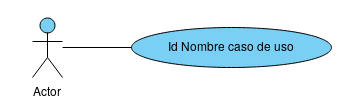
\includegraphics[width=.4\textwidth]{LIT/ActorUC}
	\end{center}
	\label{fig:acUC}
	\caption{Interacción del actor con el caso de uso}
\end{figure}

Los casos de uso se encontrarán dentro de paquetes (representados por carpetas) indicando así que pertenecen a un mismo módulo como se muestra en la figura \ref{fig:pack}.

\begin{figure}[hbtp!]
	\begin{center}
		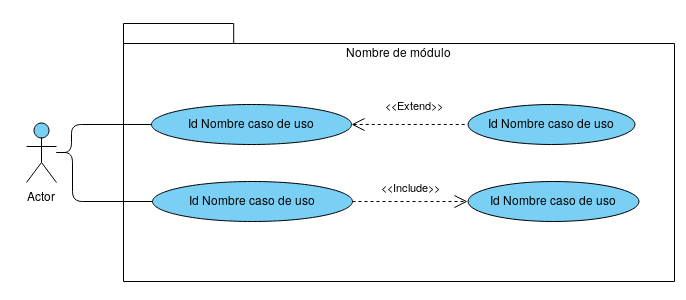
\includegraphics[width=.7\textwidth]{LIT/Paquete}
	\end{center}
	\label{fig:pack}
	\caption{Un Actor con varios caso de uso dentro de un módulo}
\end{figure}

\pagebreak
\subsection{Diagrama de casos de uso Sprint 3}
\begin{figure}[hbtp!]
	\begin{center}
		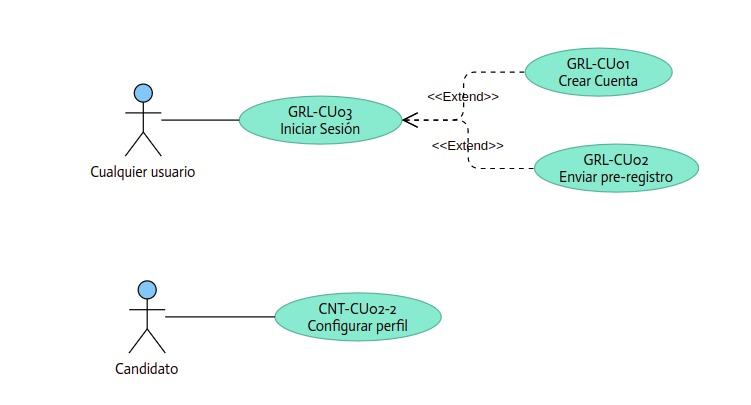
\includegraphics[width=.5\textwidth]{propuesta/imagenes/sprint3.jpeg}
	\end{center}
	\label{fig:acUC}
	\caption{Interacción del actor con el caso de uso}
\end{figure}

\subsection{Diagrama de casos de uso Sprint 4}
\begin{figure}[hbtp!]
	\begin{center}
		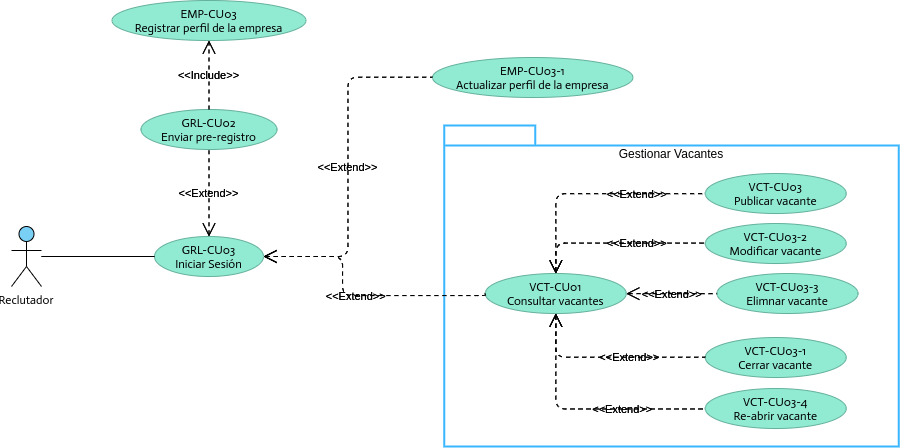
\includegraphics[width=.5\textwidth]{propuesta/imagenes/sprin4R.png}
	\end{center}
	\label{fig:acUC}
	\caption{Interacción del actor con el caso de uso}
\end{figure}

\subsection{Diagrama de casos de uso Sprint 5}
\begin{figure}[hbtp!]
	\begin{center}
		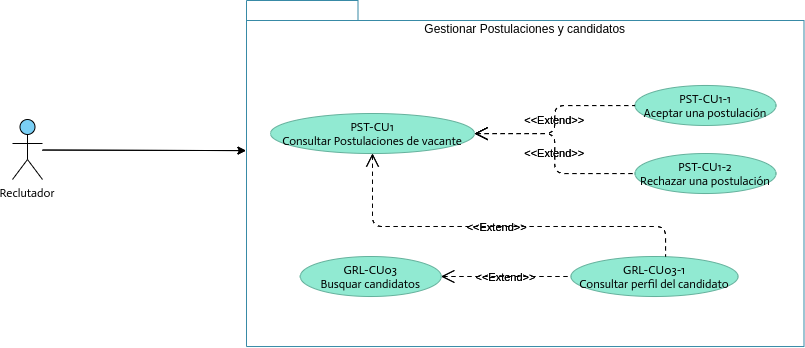
\includegraphics[width=.5\textwidth]{propuesta/imagenes/Sprint5.png}
	\end{center}
	\label{fig:acUC}
	\caption{Interacción del actor con el caso de uso}
\end{figure}


%---------------------------------------------------------
\subsection{Modelado de casos de uso}
A continuación se listas los componentes que conformam un caso de uso completo las cuales se pueden consultar en
el apendice de este documento.

\subsubsection{Modelo de estados}

Diversas entidades en el sistema  que tienen un comportamiento dinámico en el sistema, 
los que se consideraron en el desarrollo del sistema y ameritaban ser modelados a través de una 
maquina de estados.\\

\subsubsection{Actores del sistema}
 Se definen los actores identificados como participantes en los procesos del sistema. 
 Estos actores son los encargados de llevar a cabo determinadas tareas dentro de cada proceso.\\

 \subsubsection{Reglas de negocio}

 Se van describir las reglas de negocio identificadas en el sistema las cuales son una condición que 
 se debe satisfacer cuando se realiza una actividad de negocio.\\
 \subsubsection{Reglas del sistema ???}
 
\subsubsection{Casos de uso}

Las funcionalidades del sistema son representadas mediante casos de uso. Un caso de uso es una transacción entre un actor y el sistema que tiene un valor agregado o un propósito para que el actor las realice. Los casos de uso se modelan a partir de dos elementos: un aa de casos de uso y la
descripción del caso de uso.\\



\subsubsection{Mensajes del sistema}

Los mensajes se refieren a todos aquellos avisos que el sistema muestra al actor para comunicar la ocurrencia de algún evento tal como un error o una operación exitosa. 

